Springhead\KLUDGE をダウンロードしてから使えるようにするまでの流れを説明します.

\section{\KLUDGE ダウンロード}

Springhead\KLUDGE のウェブサイト\url{http://springhead.info/wiki/}\KLUDGE からzip\KLUDGE アーカイブをダウンロードできます.
\KLUDGE ただし,アーカイブの更新は必ずしも頻繁ではありません (\KLUDGE よくないことですが) \KLUDGE ので,最新のコードが入手できない可能性があります.
\KLUDGE 常に最新のコードを使用したい人は,次に説明するSubversion\KLUDGE レポジトリからコードを入手してください.

\section{SVN\KLUDGE から入手する}

Springhead\KLUDGE はSubversion\KLUDGE を用いてバージョン管理を行っています.
\KLUDGE この文書の執筆時点でSpringhead\KLUDGE のSubversion\KLUDGE レポジトリは
\begin{align*}
\text{\url{http://springhead.info/spr2/Springhead2/trunk}}
\end{align*}
\KLUDGE です.
\KLUDGE レポジトリからのコードのダウンロードは任意のユーザが行えますが,
\KLUDGE コードをコミットするには開発者として登録されている必要があります.

%Subversion\KLUDGE によるコードの入手方法については\url{http://springhead.info/wiki/}\KLUDGE にて解説されていますのでそちらを参照して下さい.

\section{\KLUDGE 開発環境}

Springhead\KLUDGE は処理系非依存の思想のもとで開発されています.
\KLUDGE このため,原理的にはWindows, Max, Unix\KLUDGE などの多くの処理系で動作するはずです.
\KLUDGE しかしながら,ほとんどの開発メンバーがWindows\KLUDGE 上のVisual Studio\KLUDGE を用いて開発を行っているため,それ以外の環境で問題無く動作する保証は残念ながらありません (\KLUDGE 多分動かないでしょう)\KLUDGE .
\KLUDGE したがって,現状ではユーザーにもWindows + Visual Studio\KLUDGE という環境での使用を推奨します.
Windows\KLUDGE やVisual Studio\KLUDGE のバージョンについては,Windows 7/8/10, Visual Studio 2015\KLUDGE では問題なく動作します.

\section{\KLUDGE ライブラリのビルド}
\label{libbuild}

\KLUDGE 以下では,Springhead\KLUDGE を保存したディレクトリを\path{C:\Springhead2}\KLUDGE と仮定して話を進めます.
Springhead\KLUDGE を入手したら,まずライブラリをビルドします.
\KLUDGE ただし,サンプルプログラムをビルドする場合に限りここでの作業は不要です (\KLUDGE ライブラリは自動的に作成されます)\KLUDGE .

\KLUDGE まず,Visual Studio\KLUDGE で以下のソリューションファイルを開いて下さい.
\begin{align*}
\text{\path{C:\Springhead2\src\Springhead14.0.sln}}
\end{align*}

\begin{center}\framebox{\footnotesize{%
\begin{minipage}{0.9\hsize}
\KLUDGE 【補足】 \KLUDGE ファイル名末尾の数字は Visual Studio \KLUDGE のバージョン番号を示しています.
\KLUDGE ただし,Visual Studio 2010 \KLUDGE より古いバージョンについてはメジャーバージョン番号のみです.
\KLUDGE その他のソリューションファイル,プロジェクトファイルも同様の規則でナンバリングしてあります.
Visual Studio 2013 \KLUDGE より以前の Visual Studio \KLUDGE を使用する場合には適宜読み替えてください.
\end{minipage}
}}\end{center}


\begin{figure}[t]
\begin{center}
\includegraphics[width=.6\hsize]{fig/libbuild.eps}
\end{center}
\caption{Building the library}
\label{fig_libbuild}
\end{figure}
\KLUDGE ソリューションを開いたらFig.\,\ref{fig_libbuild}\KLUDGE に示すように\url{Springhead}\KLUDGE プロジェクトをビルドしてください.
\KLUDGE ビルドに成功したら\path{C:\Springhead2\lib\win32\}\KLUDGE または\path{C:\Springhead2\lib\win64\}\KLUDGE ディレクトリにライブラリファイルが作成されるはずです.

Table\,\ref{table_solution_config} \KLUDGE に示すように,ビルドの設定ごとに異なるいくつかの構成が用意されています.
\KLUDGE ユーザアプリケーションの都合に合わせて使い分けてください.

\begin{table}[t]
\caption{Build configurations}
\label{table_solution_config}
\begin{center}
\begin{tabular}{lll}
\toprule
\KLUDGE 構成名				& \KLUDGE ビルド設定					& \KLUDGE 作成されるライブラリファイル名	\\ \midrule
\url{Release}		& multithread, DLL				& \url{Springhead14.0\# \#.lib}	    \\
\url{Debug}			& multithread, Debug, DLL		& \url{Springhead14.0\# \#D.lib}	\\
\url{Trace}			& multithread, Debug, DLL		& \url{Springhead14.0\# \#T.lib}	\\ \bottomrule
\multicolumn{3}{l}
{\footnotesize{%
\vbox{\vbox to 1mm{}
      \hbox{\KLUDGE ・ \url{\# \#} \KLUDGE はプラットフォームを表す \url{Win32} \KLUDGE 又は \url{x86} \KLUDGE となります.}
      \hbox{\KLUDGE ・ \url{Trace} \KLUDGE 構成とは,フレームポインタ情報付き \url{Release} \KLUDGE 構成のことです.}}}}
\end{tabular}
\end{center}
\end{table}

\begin{center}\framebox{\footnotesize{%
\begin{minipage}{0.9\hsize}
\KLUDGE 【補足】 \KLUDGE ライブラリファイルのビルド設定及び名称はこれまでの開発経緯による理由で,少々複雑になっています.
\begin{itemize}
\item{Visual Studio 2008 \KLUDGE では,すべての構成が Static Link \KLUDGE 設定です.}
\item{Visual Studio 2010 \KLUDGE では, \url{Release} / \url{Debug} \KLUDGE 構成が Static Link \KLUDGE 設定,
\url{ReleaseDll} / \url{DebugDll} / \url{Trace} \KLUDGE 構成が DLL \KLUDGE 設定です.}
\item{Visual Studio 2012 \KLUDGE では,すべての構成が DLL \KLUDGE 設定です.}
\item{Visual Studio 2010 \KLUDGE 以前のバージョンでは,プラットフォームが 32\KLUDGE ビットの場合,ライブラリファイル名に \url{Win32} \KLUDGE が付きません.}
\item{Visual Studio 2010 \KLUDGE の \url{ReleaseDll} \KLUDGE 構成及び \url{DebugDll} \KLUDGE 構成では,\url{.lib} \KLUDGE の前にそれぞれ
\url{M} \KLUDGE 及び \url{MD} \KLUDGE が付きます.}
\end{itemize}
\end{minipage}
}}\end{center}


\section{\KLUDGE サンプルプログラムのビルド}

\KLUDGE サンプルプログラムをビルドするには
\begin{align*}
\text{\path{C:\Springhead2\src\Samples\All14.0.sln}}
\end{align*}
\KLUDGE を開きます.
\KLUDGE ビルドしたいサンプルをスタートアッププロジェクトに設定し,ビルド,実行してください.

\KLUDGE 残念なことですが,すべてのサンプルプログラムが問題なく動作する状態には維持されていません.
\url{Physics/BoxStack}\KLUDGE や\url{Physics/Joints}\KLUDGE が比較的良くメンテナンスされていますので試してみてください.

\KLUDGE 実行時にDLL\KLUDGE が見つからないためにエラーが起こるかもしれません。
\begin{align*}
\text{\path{Springhead2\bin\win32}}
\text{\path{Springhead2\bin\win64}}
\end{align*}
\KLUDGE にPath\KLUDGE を通してください。

\section{\KLUDGE アプリケーションの作成}
\label{sec_create_application}

\begin{figure}[t]
\begin{center}
\includegraphics[width=.6\hsize]{fig/newproject1.eps}
\end{center}
\caption{Create new project}
\label{fig_newproject1}
\end{figure}

\begin{figure}[t]
\begin{center}
\includegraphics[width=.6\hsize]{fig/newproject2.eps}
\end{center}
\caption{Project configuration}
\label{fig_newproject2}
\end{figure}

\begin{figure}[t]
\begin{center}
\includegraphics[width=.6\hsize]{fig/newproject3.eps}
\end{center}
\caption{Create source file}
\label{fig_newproject3}
\end{figure}

Springhead\KLUDGE を使って簡単なアプリケーションプログラムを作成する道筋を説明します.
\KLUDGE 以下ではVisual Studio 2013\KLUDGE を想定します.

\subsection*{\KLUDGE プロジェクトの作成}

\KLUDGE 「Visual C++ Win32\KLUDGE プロジェクト」を作成します.作成するディレクトリを \path{C:\Experiments} \KLUDGE と仮定します. \KLUDGE 他のディレクトリに作成する場合には,プロジェクトに指定するインクルードファイル及びライブラリファイルのパスが,保存した Springhead \KLUDGE を正しく参照するように注意してください. \KLUDGE プロジェクト名は好きな名前を付けてください.アプリケーションの設定で「コンソールアプリケーション」を選び,空のプロジェクトをチェックします.

\KLUDGE プロジェクトを作成したら「プロジェクト $>$ \KLUDGE 新しい項目の追加 $>$ C++\KLUDGE ファイル(.cpp)\KLUDGE 」としてソースファイルを作成します.
\KLUDGE ここでは仮に\url{main.cpp}\KLUDGE とします.

\subsection*{\KLUDGE ソースコードの編集}

\begin{table}[t]
\caption{Simplest program code}
\label{table_simplest_code}
{\small
\begin{sourcecode}
#include <Springhead.h>
#include <Framework/SprFWApp.h>
using namespace Spr;

class MyApp : public FWApp{
public:
    virtual void Init(int argc = 0, char* argv[] = 0){
        FWApp::Init(argc, argv);

        PHSdkIf* phSdk = GetSdk()->GetPHSdk();
        PHSceneIf* phscene = GetSdk()->GetScene()->GetPHScene();
        CDBoxDesc bd;
        
        // 床を作成
        PHSolidIf* floor = phscene->CreateSolid();
        floor->SetDynamical(false);
        bd.boxsize = Vec3f(5.0f, 1.0f, 5.0f);
        floor->AddShape(phSdk->CreateShape(bd));
        floor->SetFramePosition(Vec3d(0, -1.0, 0));
    
        // 箱を作成
        PHSolidIf* box = phscene->CreateSolid();
        bd.boxsize = Vec3f(0.2f, 0.2f, 0.2f);
        box->AddShape(phSdk->CreateShape(bd));
        box->SetFramePosition(Vec3d(0.0, 1.0, 0.0));

        GetSdk()->SetDebugMode(true);
    }
} app;

int main(int argc, char* argv[]){
    app.Init(argc, argv);
    app.StartMainLoop();
    return 0;
}
\end{sourcecode}
}
\end{table}

\KLUDGE 作成した\url{main.cpp}\KLUDGE にTable\,\ref{table_simplest_code}\KLUDGE に示すコードを書き込んでください.これがSpringhead\KLUDGE を使用した (\KLUDGE ほぼ) \KLUDGE 最小のプログラムコードです.

\section*{\KLUDGE プロジェクト設定}

\begin{figure}[t]
\begin{center}
\includegraphics[width=.6\hsize]{fig/newproject4.eps}
\end{center}
\caption{Add include path}
\label{fig_newproject4}
\end{figure}

\begin{figure}[t]
\begin{center}
\includegraphics[width=.6\hsize]{fig/newproject5.eps}
\end{center}
\caption{Add library path}
\label{fig_newproject5}
\end{figure}

\begin{figure}[t]
\begin{center}
\begin{tabular}{c}
\includegraphics[width=.6\hsize]{fig/newproject6_truncate.eps} \\
\includegraphics[width=.6\hsize]{fig/newproject7_truncate.eps}
\end{tabular}
\end{center}
\caption{Specify library file}
\label{fig_newproject6}
\end{figure}

\begin{figure}[t]
\begin{center}
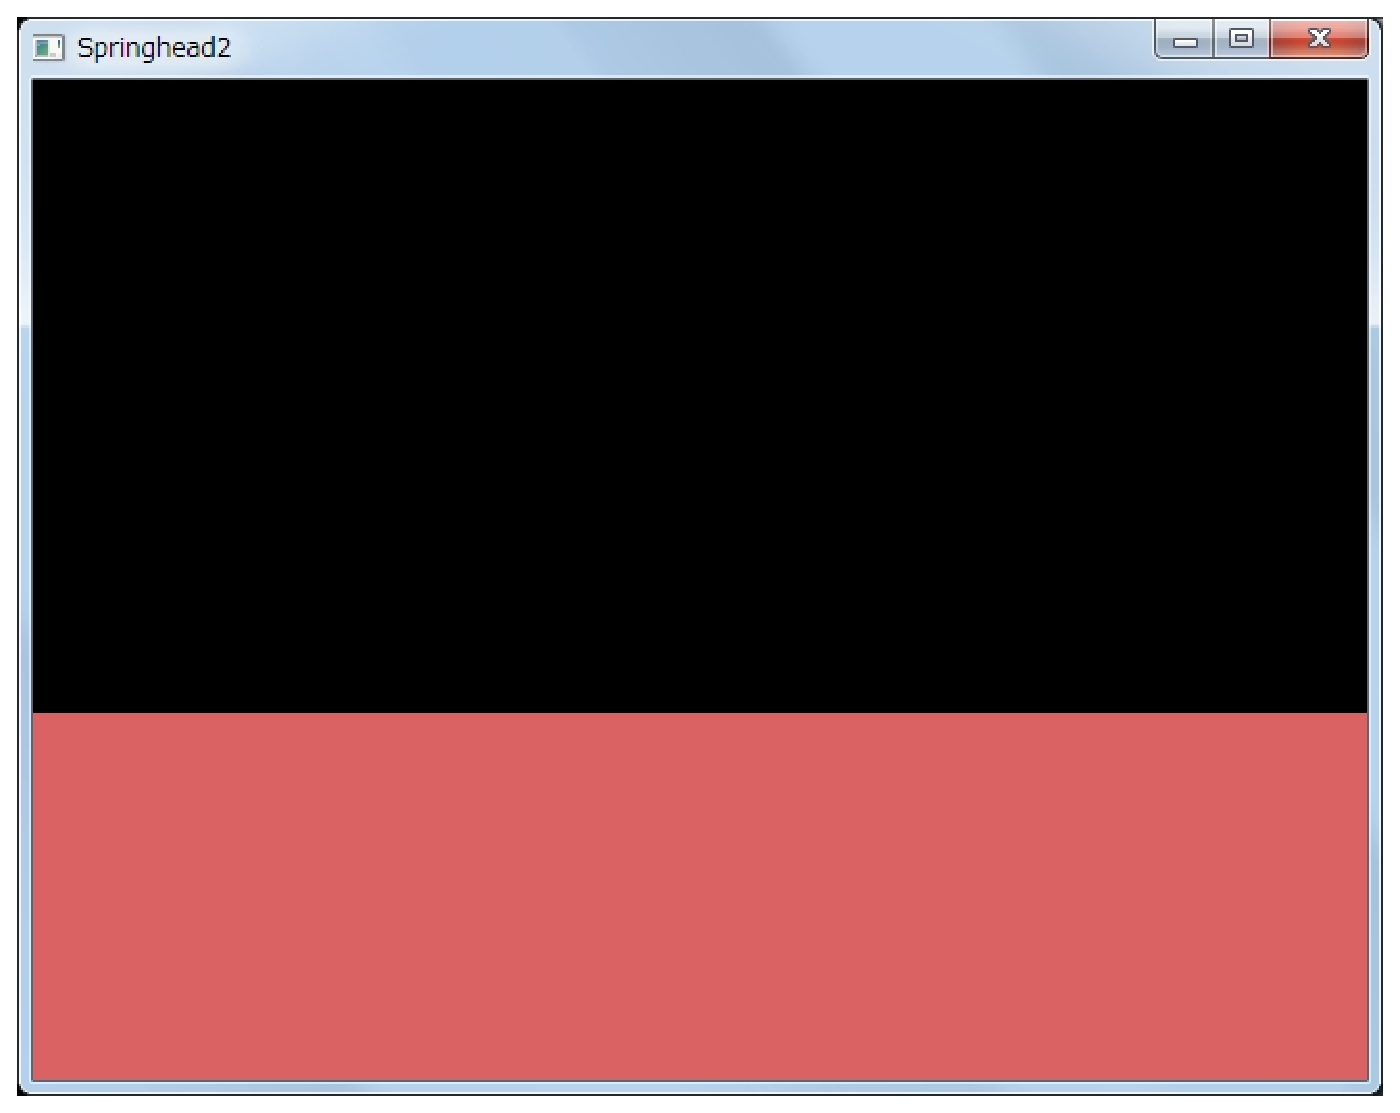
\includegraphics[width=.6\hsize]{fig/newproject8.eps}
\end{center}
\caption{Program running}
\label{fig_newproject8}
\end{figure}

\KLUDGE ビルドするまえにいくつかのプロジェクト設定が必要です.
64\KLUDGE ビットプラットフォームを使用する場合には,プロパティーページの「構成マネージャー」で「\url{x64}\KLUDGE 」プラットフォームを新規作成して選択しておきます.
\KLUDGE また,\ref{libbuild} \KLUDGE で説明したライブラリのビルドは済んでいるものとします.

\KLUDGE まずプロジェクトのプロパティページを開き,構成を「すべての構成」としてください.
\KLUDGE 次に「C/C++ $>$ \KLUDGE 全般 $>$ \KLUDGE 追加のインクルードディレクトリ」に,Fig.\,\ref{fig_newproject4}\KLUDGE のようにSpringhead\KLUDGE のインクルードファイルへのパスを指定してください.
\KLUDGE さらに,「リンカー $>$ \KLUDGE 全般 $>$ \KLUDGE 追加のライブラリディレクトリ」にFig.\,\ref{fig_newproject5}\KLUDGE のようにSpringhead\KLUDGE のライブラリファイルへのパスを指定します (64\KLUDGE ビット構成ぼ場合は \url{win32} \KLUDGE の代わりに \url{win64} \KLUDGE を指定します)\KLUDGE .

\KLUDGE 今度は構成を「Debug\KLUDGE 」にします.
\KLUDGE 「C/C++ $>$ \KLUDGE コード生成 $>$ \KLUDGE ランタイムライブラリ」を「マルチスレッド \KLUDGE デバッグ DLL (\url{/MDd})\KLUDGE 」にします.
\KLUDGE 次に「リンカー $>$ \KLUDGE 入力 $>$ \KLUDGE 追加の依存ファイル」に\url{Springhead14.0DWin32.lib}\KLUDGE を追加してください.

\KLUDGE 最後に構成を「Release\KLUDGE 」に切り替えて同様の設定をします.
\KLUDGE ランタイムライブラリを「マルチスレッド DLL (\url{/MD})\KLUDGE 」として,追加の依存ファイルに\url{Springhead14.0Win32.lib}\KLUDGE を追加します.

\section*{\KLUDGE ビルド・実行}

\KLUDGE 以上で準備完了です.ビルド(F7)\KLUDGE して,実行(F5)\KLUDGE してみてください.
Fig.\,\ref{fig_newproject8}\KLUDGE のような画面が出てくれば成功です.
